\chapter{Estado del arte}


%=========================================================
%                                                         Estado del arte
%=========================================================
%\section{Estado del arte}
\noindent En esta sección se describen las aplicaciones web existentes en el mercado que se apeguen con el tema del presente Trabajo Terminal, esto con la finalidad de saber si existe una aplicación que cubra con los problemas que atañe este trabajo terminal o en su defecto, ver que caracteristicas se pueden tomar como base o mejorar y así dar solución a los problemas que ataca el proyecto. 


%=========================================================
%                                                         Historia
%=========================================================
%\section{Historia}


%=========================================================
%                                                         Aplicaciones
%=========================================================
\section{Aplicaciones}
\noindent Dentro de la investigación que se realizó con respecto a sistemas o aplicaciones web que tuviesen el mismo objetivo al proyecto propuesto. A continuación se muestran las aplicaciones que se encontraron, así como una descripción de su funcionamiento y las principales caracteristicas de cada una de ellas.
\subsection{Aplicaciones Tournament Software}
\noindent Esta aplicación ofrece al usuario un plataforma en la que puede registrar equipos deportivos, a su vez le ofrece crear ligas (competencias) entre los equipos que previamente registro, agregando que al final le dará una tabla de posiciones de los equipos y si este desea ver más información de uno en particular, desglosar la información en otra vista. \cite{ts}
Características: 
\begin{itemize}
	\item Login: Necesario para que el coordinador de los equipos registren los equipos que dirigen.
	\item Registro de equipos: Necesario para poder generar eventos entre los equipos registrados.
	\item Creación de eventos: Se necesita tener equipos registrados para poder eventos entre los distintos equipos.
	\item Consulta de resultados: Una vez concluido los eventos, da la opción de registrar los resultados para su consulta.
\end{itemize}
\pagebreak
%=========================================================
%                                                         Imagenes
%=========================================================
\begin{figure}[h]
	\centering
	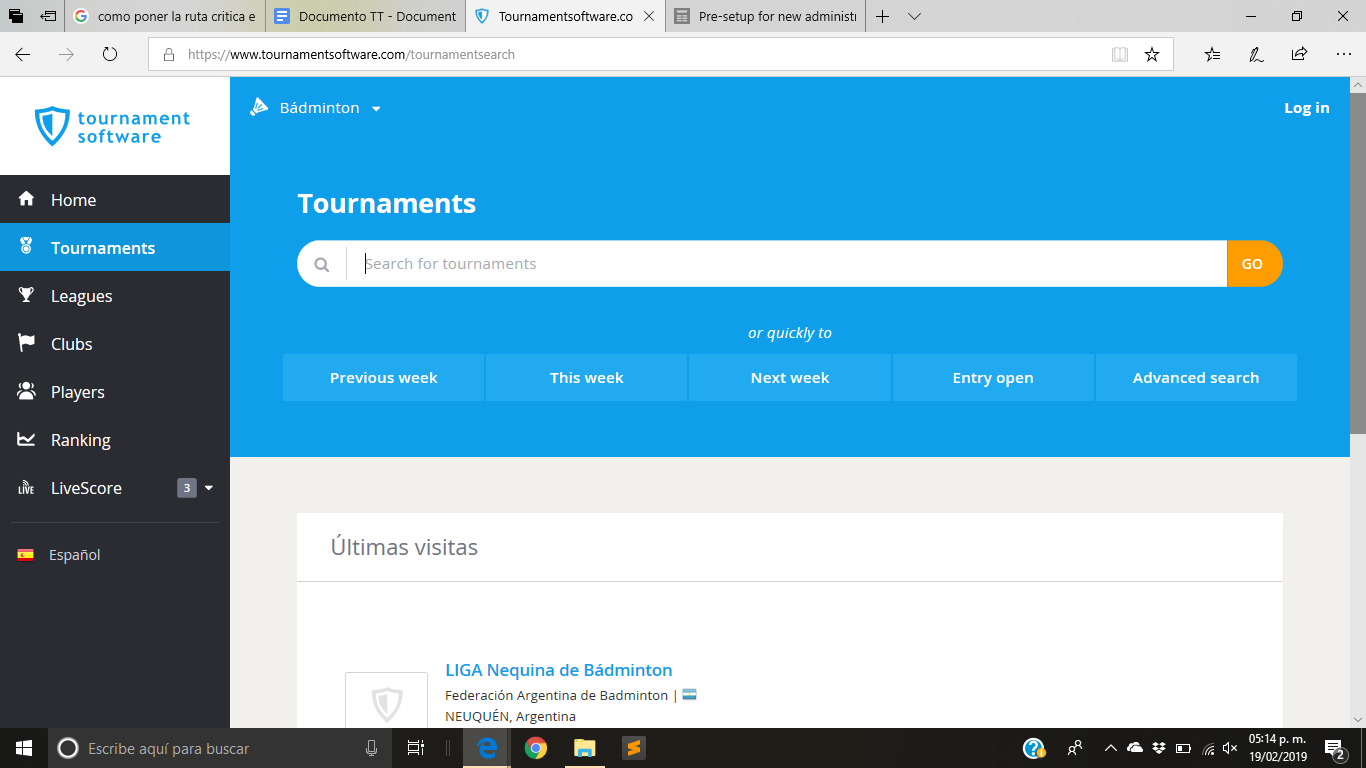
\includegraphics[width=12cm, height=6cm]{Imagenes/Aplicaciones/ToS1.png}
	\caption{Eventos registrados}
\end{figure}
\begin{figure}[h]
	\centering
	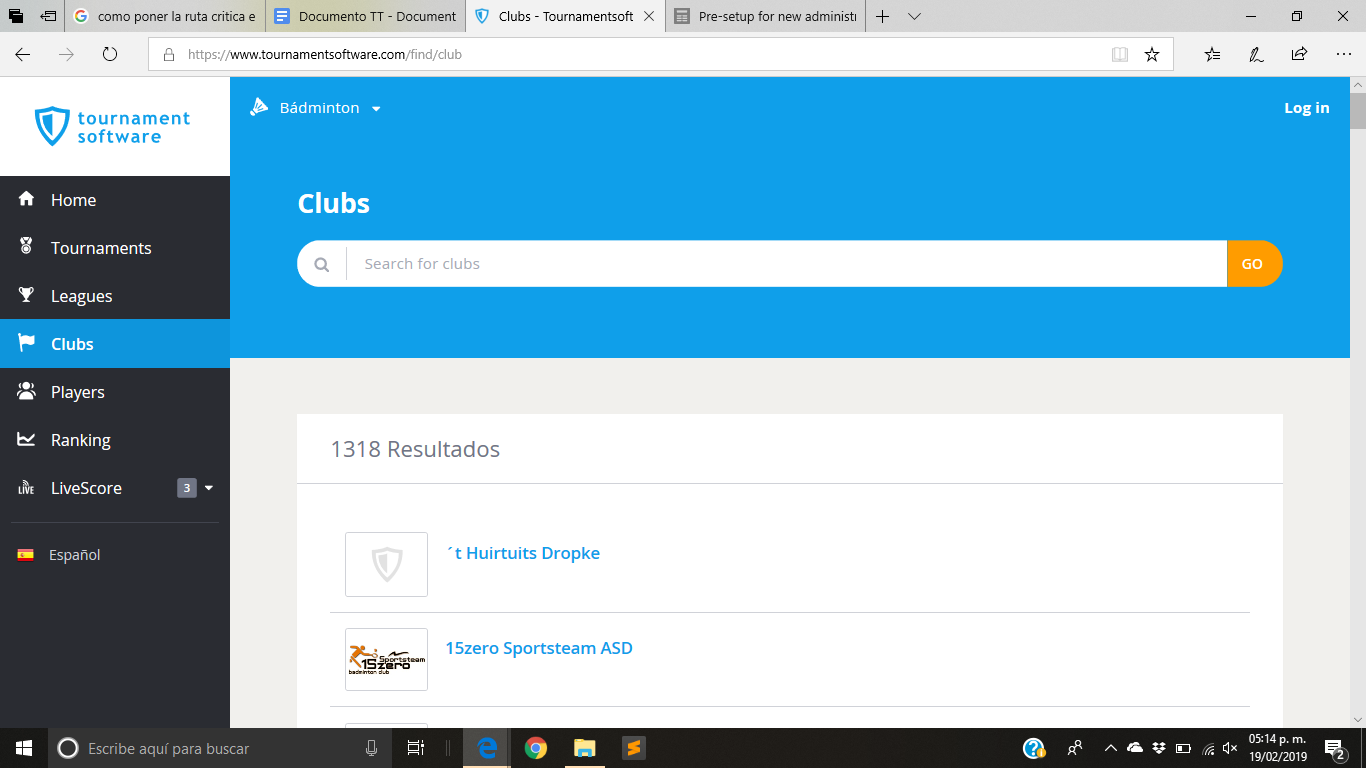
\includegraphics[width=12cm, height=6cm]{Imagenes/Aplicaciones/ToS2.png}
	\caption{Clubs registrados}
\end{figure}
\pagebreak
\begin{figure}[h]
	\centering
	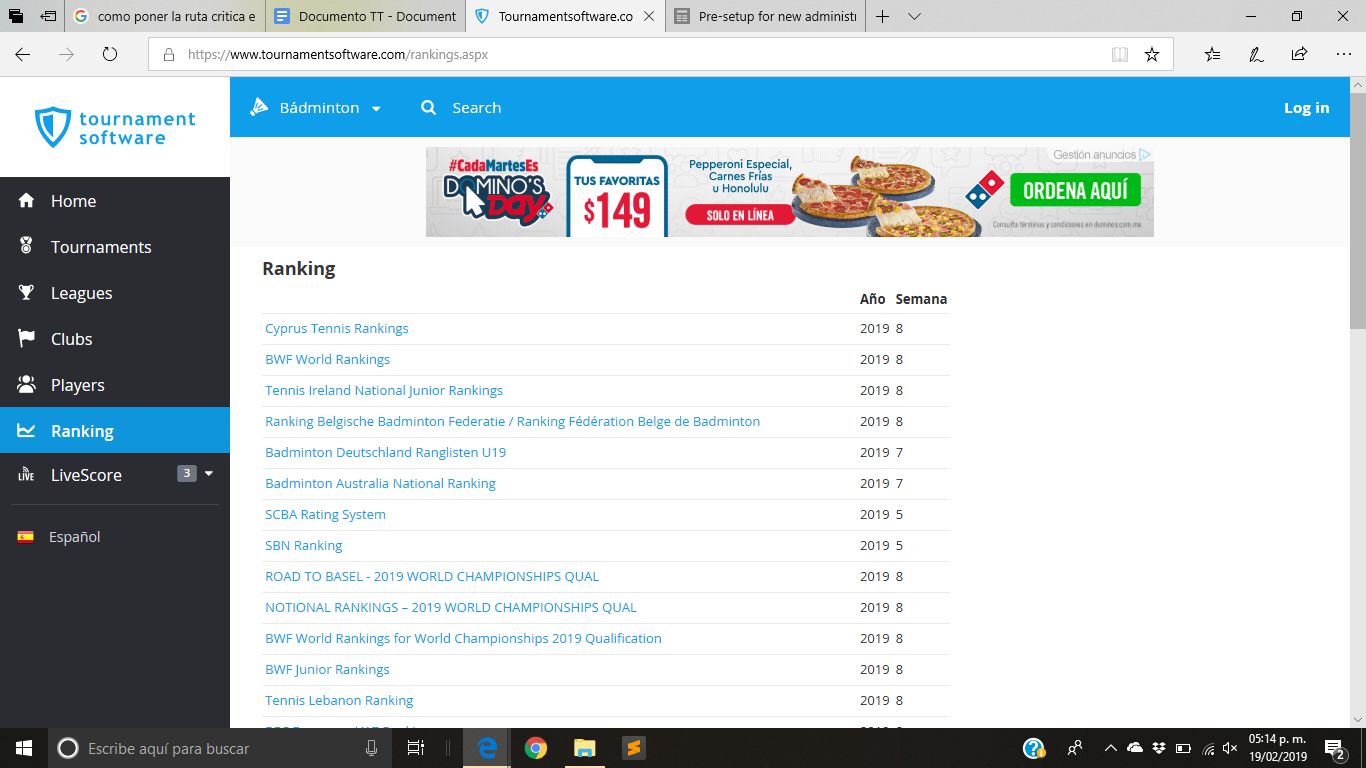
\includegraphics[width=12cm, height=6cm]{Imagenes/Aplicaciones/Tos3.png}
	\caption{Resultados}
\end{figure}

\subsection{Aplicaciones Active Network}
\noindent Esta aplicación ofrece a los usuarios de un manera organizada y fácil, el controlar alguna actividad deportiva, a su vez tienen un mercado más amplio ya que ofrecen sus servicio a escuelas, eventos deportivos, entre otros. Una desventaja que se encontró, es que para cada actividad deportiva se tiene una página designada, que es independiente al resto. \cite{act}
Características: 
\begin{itemize}
	\item Login: Necesario para poder registrar, crear eventos.
	\item Calendario: Muestra los eventos próximos previamente registrados.
	\item Registro de equipos: Permite dar de alta equipos.
	\item Reportes: Generar reportes al final de los eventos.
	\item Registro de eventos: Crea eventos que involucran a los equipos registraos.
\end{itemize}
%=========================================================
%                                                         Imagenes
%=========================================================
\begin{figure}[ht]
	\centering
	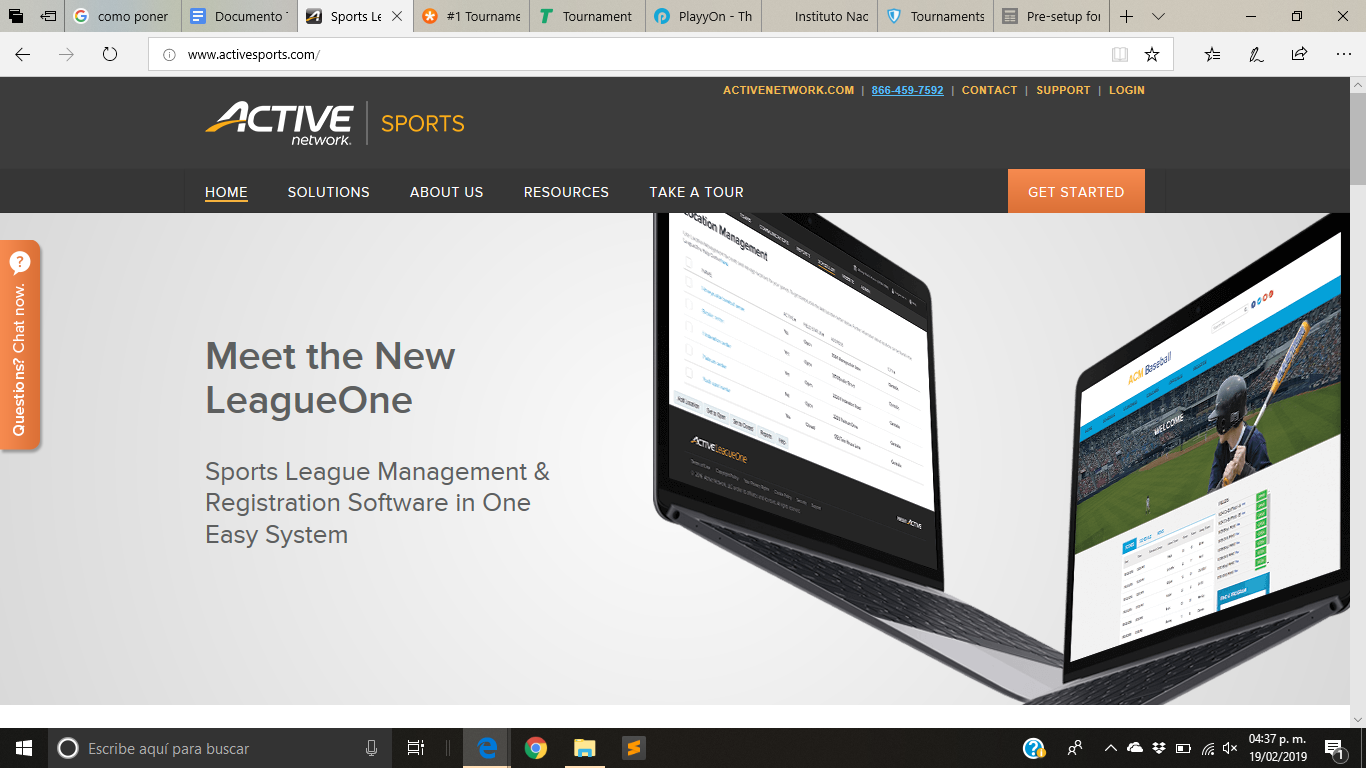
\includegraphics[width=12cm, height=6cm]{Imagenes/Aplicaciones/AN1.png}
	\caption{Página principal}
\end{figure}

\pagebreak

\begin{figure}[ht]
	\centering
	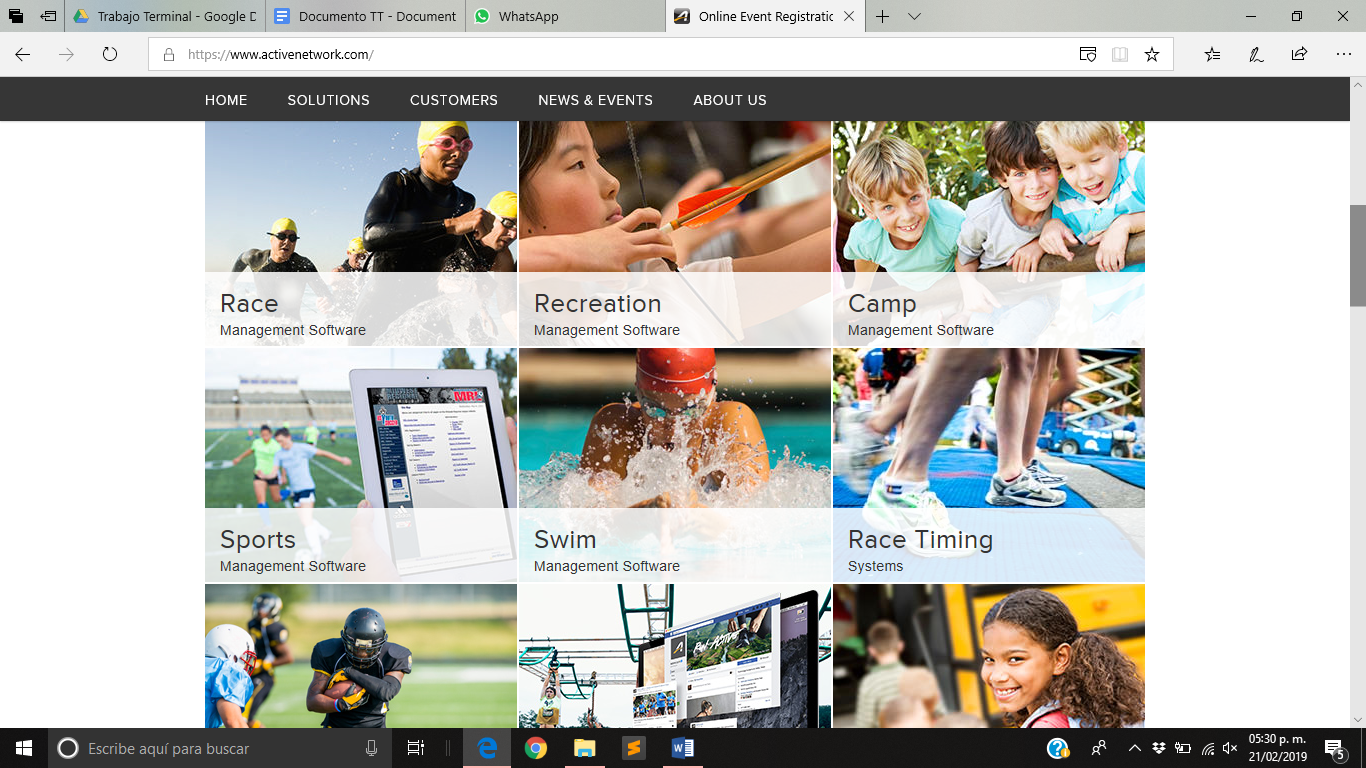
\includegraphics[width=12cm, height=6cm]{Imagenes/Aplicaciones/AN2.png}
	\caption{Eventos deportivos}
\end{figure}


\subsection{Aplicaciones TeamSnap Tournament}
\noindent La aplicación ofrece a los usuarios, un espacio en donde pueden registrar eventos deportivos, agendar o llevar control en el calendario de eventos, saber tablas de posiciones (estadísticas), otra característica de esta aplicación es que tiene un apartado en donde el administrador puede definir el precio de la inscripción a los eventos. \cite{team}
Características: 
\begin{itemize}
	\item Creación de eventos: Generar eventos para que posteriormente los interesados puedan inscribirse.
	\item Dar precio para inscripción a un evento: Permite asignar un monto monetario, si asi se desea para la inscripción a un evento.
	\item Cédula de inscripción: Permite generar el formato de inscripción para los distintos eventos.
	\item Difusión: Una vez creado un evento, se permite promocionar el evento dentro de la misma página.
\end{itemize}
%=========================================================
%                                                         Imagenes
%=========================================================
\begin{figure}[hbt]
	\centering
	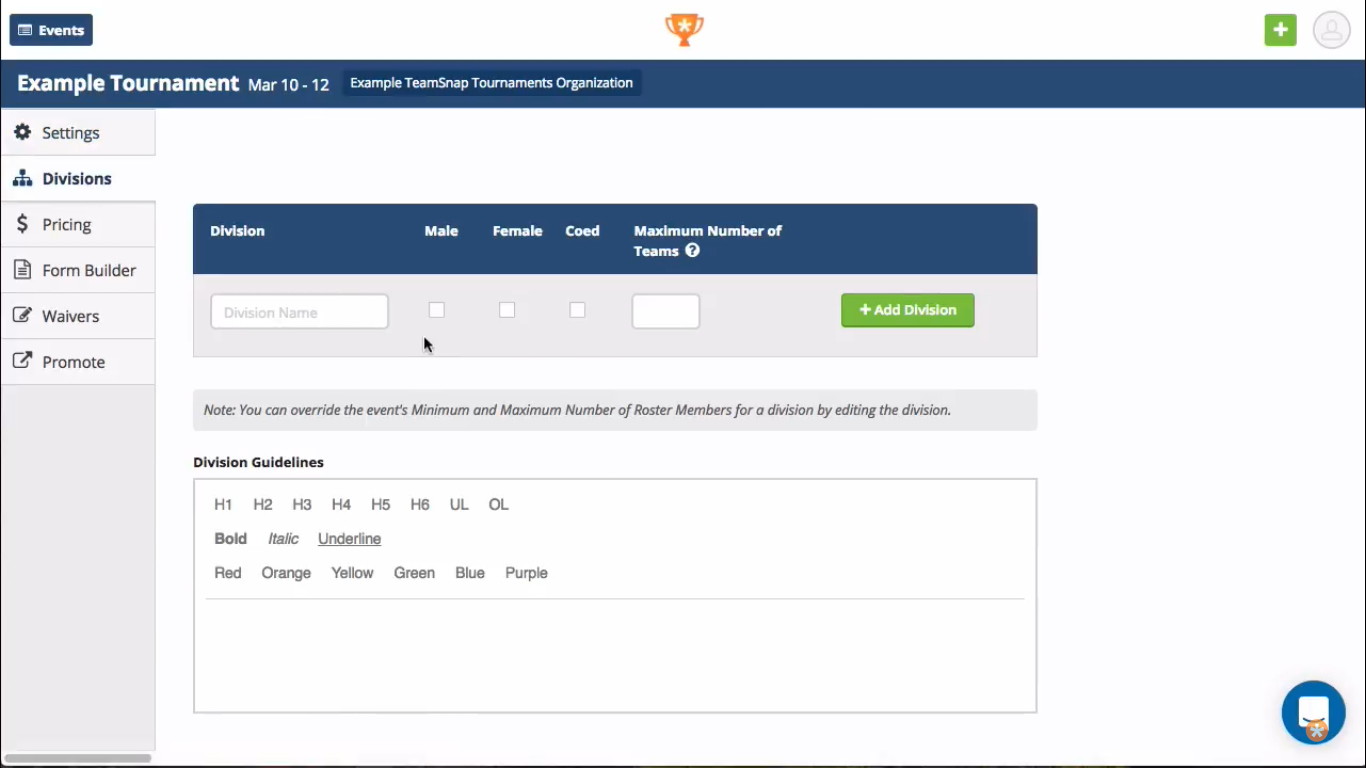
\includegraphics[width=12cm, height=6cm]{Imagenes/Aplicaciones/TsT1.png}
	\caption{Registro de competencias}
		\label{Imagen}
\end{figure}
\pagebreak
\begin{figure}[hbt]
	\centering
	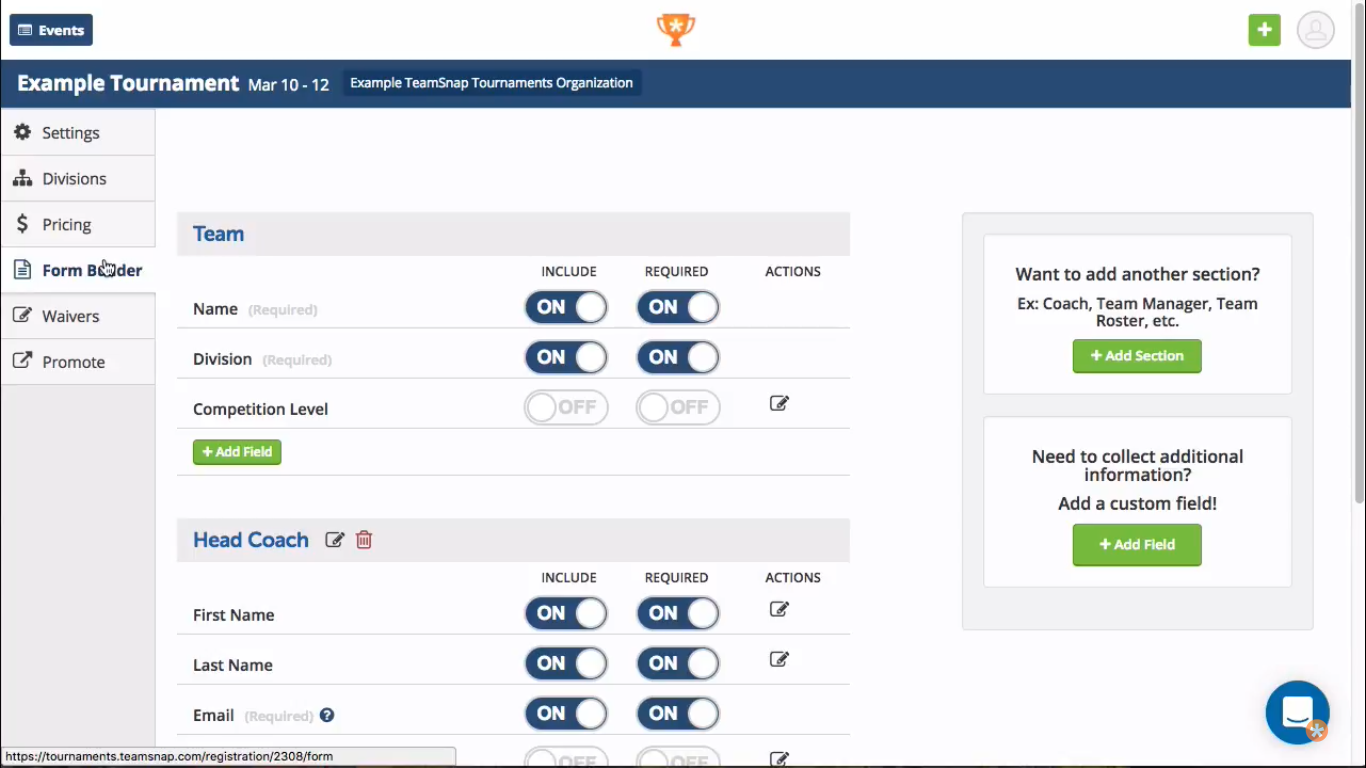
\includegraphics[width=12cm, height=6cm]{Imagenes/Aplicaciones/TsT2.png}
	\caption{Creación de cédula de inscripción}
\end{figure}
\begin{figure}[hbt]
	\centering
	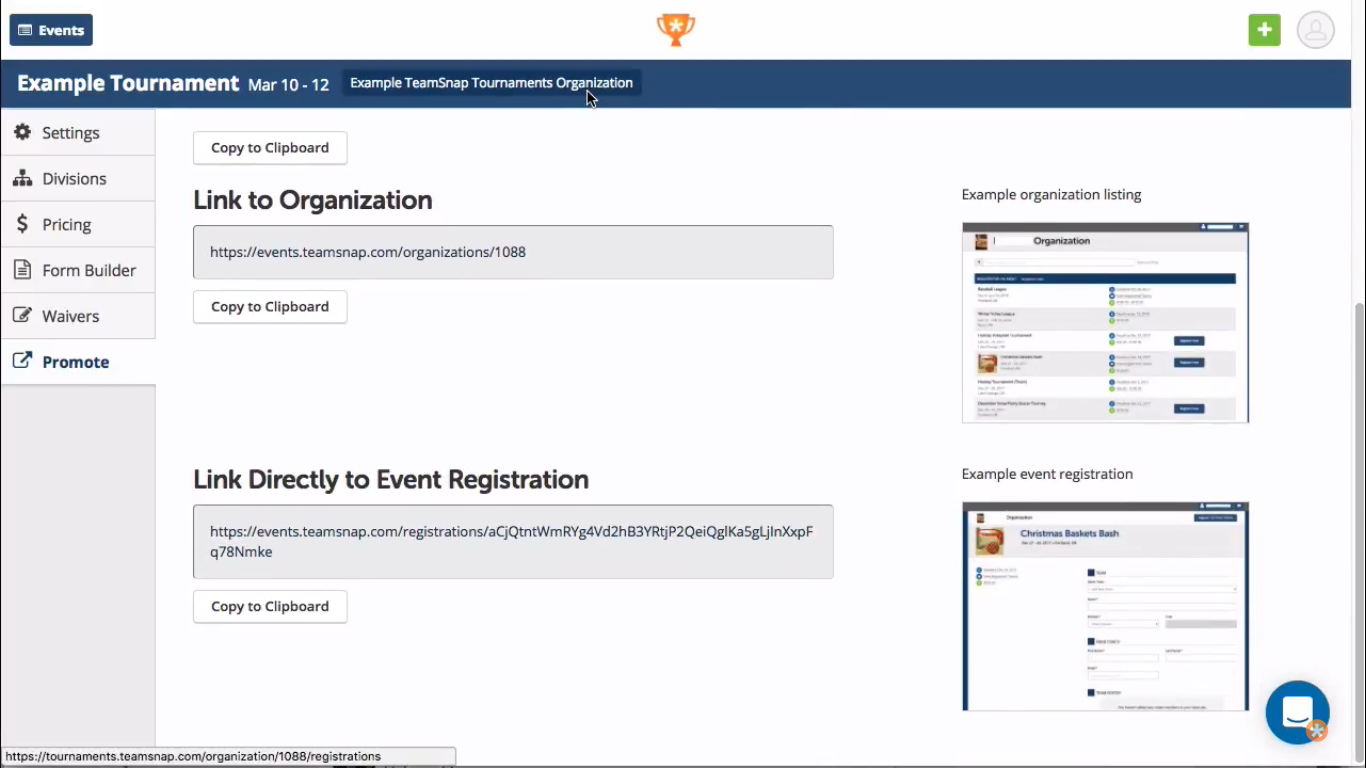
\includegraphics[width=12cm, height=6cm]{Imagenes/Aplicaciones/TsT3.png}
	\caption{Promover}
\end{figure}
\pagebreak


\subsection{Aplicaciones TorneoPal}
\noindent Esta aplicación, al igual que las anteriores, ofrece a los usuarios el generar un horario de actividades, generar torneos entre los equipos registrados y a su vez, en el apartado de estadísticas, ver en una tabla general el estatus de los equipos. \cite{tp}
Características: 
\begin{itemize}
	\item Creación de eventos: Permite crear eventos y asignar, si lo desea un límite de edad para los participantes, el número máximo de integrantes por equipo entre otras características.
	\item Resultados: Una vez concluido los eventos se puede ingresar los resultados para que puedan ser visualizados.
	\item Eliminar eventos: En caso de que se desee, se puede eliminar un evento.
	\item Cambio de equipo en categorías: Se puede modificar un evento, en este caso modificar la categoría en la que se participará.
	\item Informe a árbitros: Se le informa al personal de árbitraje de los eventos que han sido asignados.
	\item Calendario: Muestra los eventos próximos registrados.
	
\end{itemize}
%=========================================================
%                                                         Imagenes
%=========================================================
\begin{figure}[h!]
	\centering
	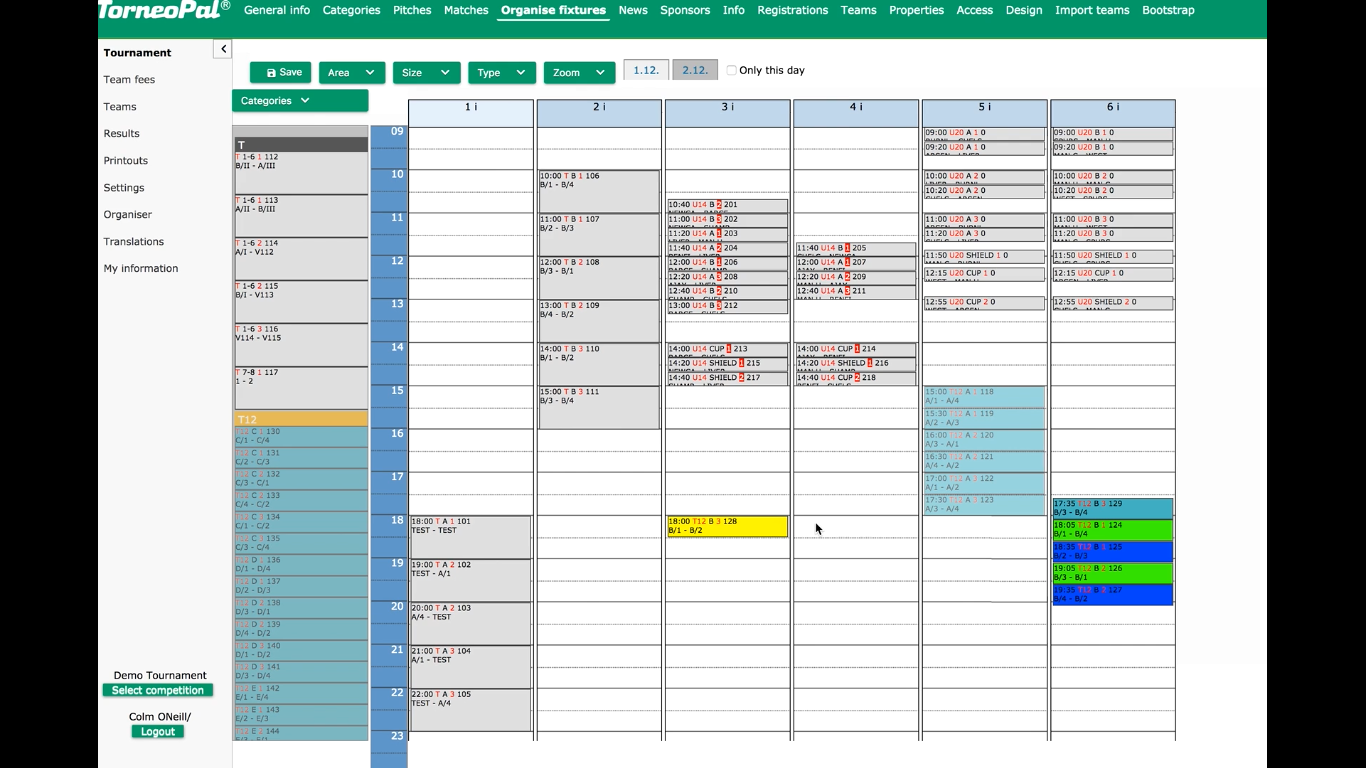
\includegraphics[width=12cm, height=6cm]{Imagenes/Aplicaciones/TP1.png}
	\caption{Calendario de eventos}
\end{figure}
\begin{figure}[h!]
	\centering
	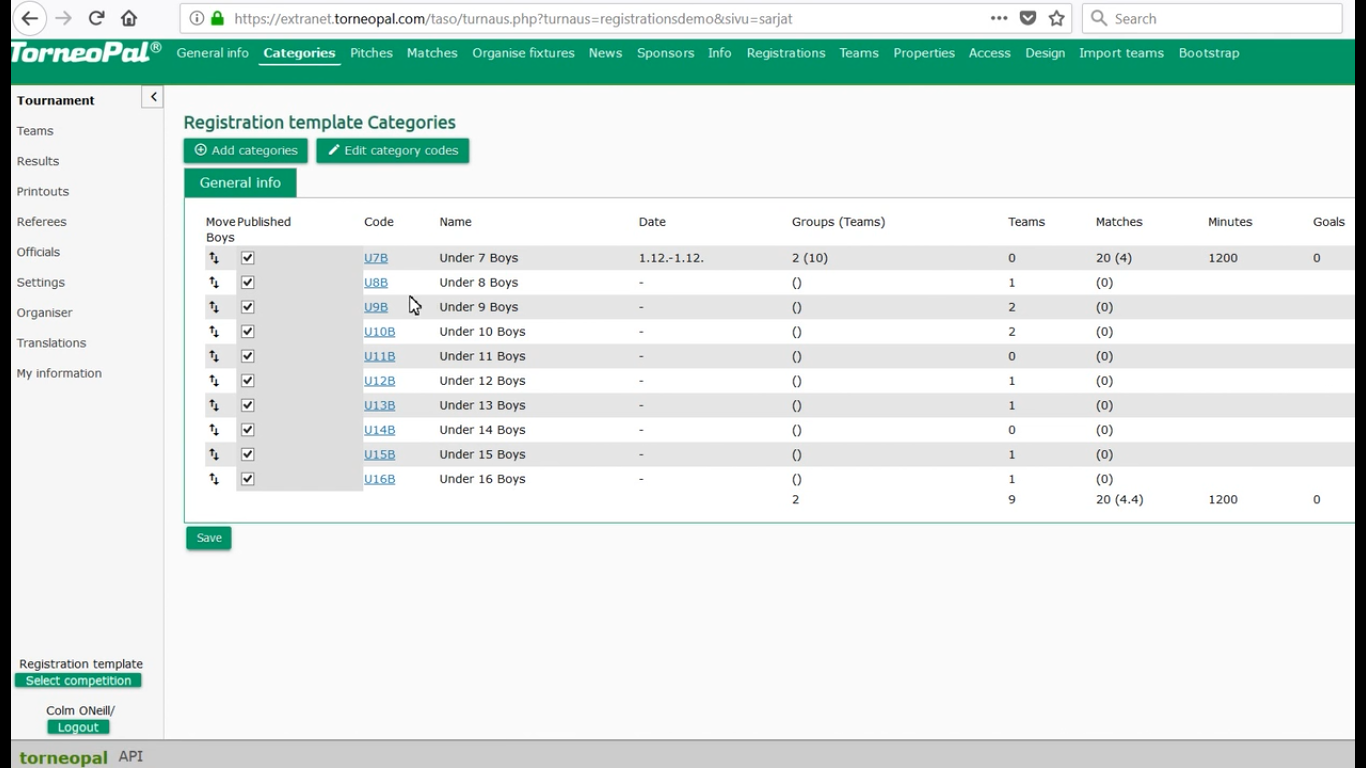
\includegraphics[width=12cm, height=6cm]{Imagenes/Aplicaciones/TP2.png}
	\caption{Registro eventos}
\end{figure}
\pagebreak

\subsection{Aplicaciones Instituto Nacional del deporte CHILE}
\noindent Esta aplicación está dirigida a un mercado en específico, ofreciendo dentro de esta un calendario de próximos eventos, registrarse en alguno del interés del usuario, como complemento se informa los requisitos para poder participar en los eventos y  un apartado en donde pueden dar de alta a organizaciones. No cuenta con un apartado donde muestre estadísticas. \cite{IND}
Características: 
\begin{itemize}
	\item Registro: Dirigido a los estudiantes que deseen participar en los eventos ya registrados.
	\item Calendario: Muestra de manera general los eventos próximos.
	\item Informes: Proporciona información general a los interesados.
	
\end{itemize}
%=========================================================
%                                                         Imagenes
%=========================================================
\begin{figure}[hbt!]
	\centering
	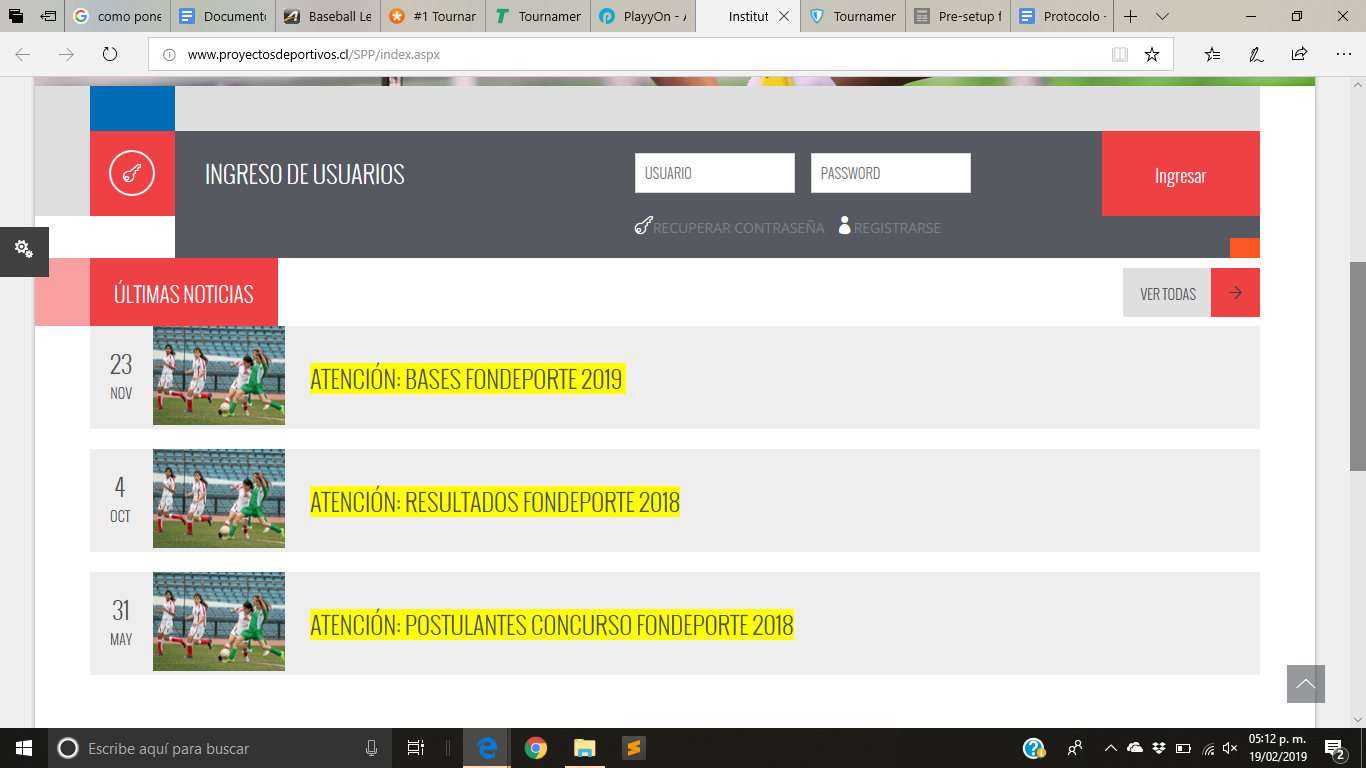
\includegraphics[width=12cm, height=6cm]{Imagenes/Aplicaciones/INDC1.png}
	\caption{Calendario de eventos}
\end{figure}
\begin{figure}[hbt!]
	\centering
	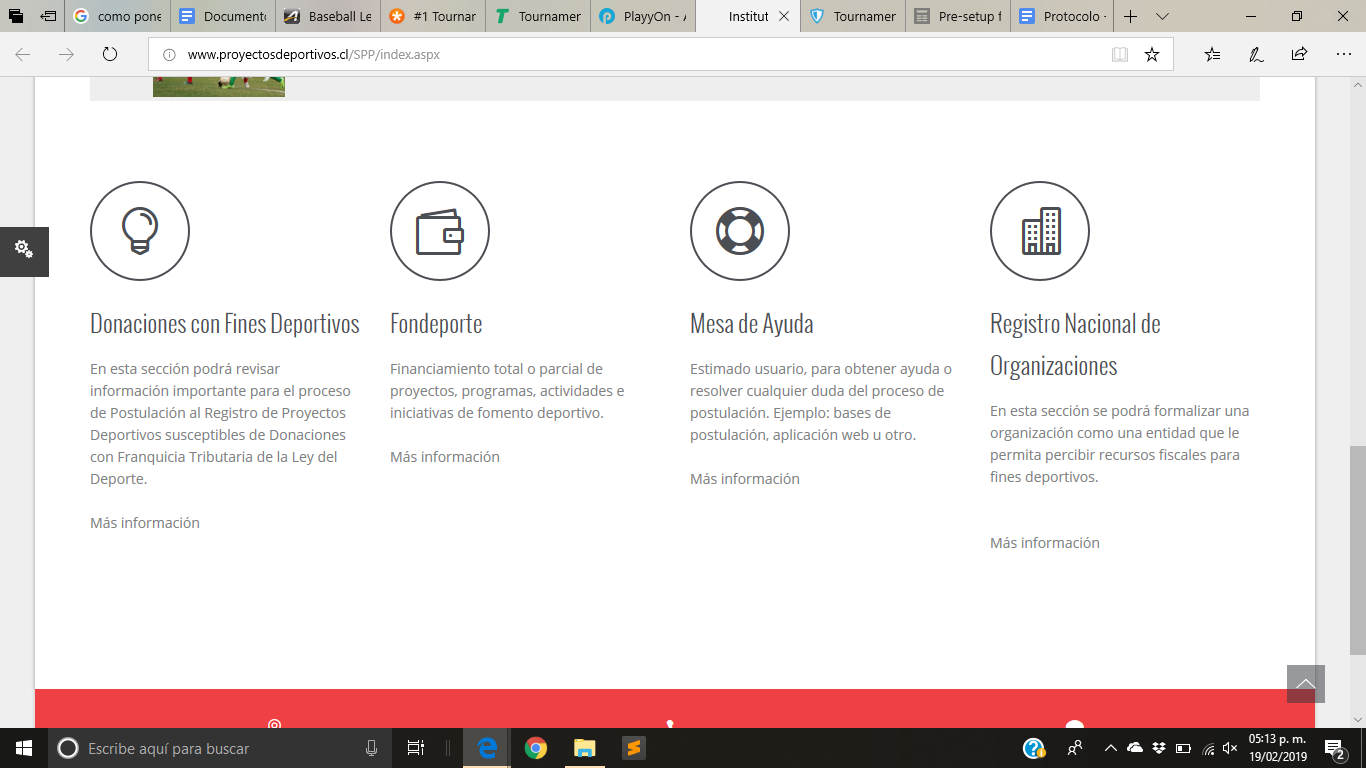
\includegraphics[width=12cm, height=6cm]{Imagenes/Aplicaciones/INDC2.png}
	\caption{Contacto}
\end{figure}
\pagebreak

\subsection{Prototipo para el registro a interpolitécnicos RIDESCOM}
\noindent Esta aplicación esta dirigida a la comunidad del Instituto Politécnico Nacional, especificamente en la Escuela Superior de Cómputo. La cual ofrece a la comunidad un espacio donde pueda ver el calendario de eventos próximos, resultados de la comunidad que participó, así como la posibilidad de inscribirse a un evento cuando estos esten disponibles. 
\\Dentro de la investigación se encontró características en común en todas las aplicaciones, que para nuestro caso en particular ayuda a atacar la problemática, sin embargo ninguna de ellas cumple con todos los requisitos que se busca, ya sea porque no cumple con todos los puntos o en algunos casos, es necesario realizar una subscripción para poder hacer uso del servicio que se ofrece. Sin embargo se puede tomar como punto de referencia algunos casos para ser implementados en nuestra aplicación.
Las características que pretende tener nuestro proyecto son las siguientes:
\begin{itemize}
	\item Registro de eventos: Crear eventos deportivos para que los interesados puedan inscribirse en estos.
	\item Calendario de eventos: Se mostrará los eventos que ya han sido registrados.
	\item Resultados: Una vez que se concluyan los eventos, podrán ingresar los resultados de los participantes para que pueda ser vistos por la comunidad escolar.
	\item Inscripción a eventos: Permitir a los alumnos interesados inscribirse en el evento de su interes. 
\end{itemize}

A continuación se muestra una página comparativa, realizando énfasis en las características principales de cada una de ellas. Para más detalles consulte la \ref{tablacomparativa}.

\begin{figure} [hbt!]
	\centering
	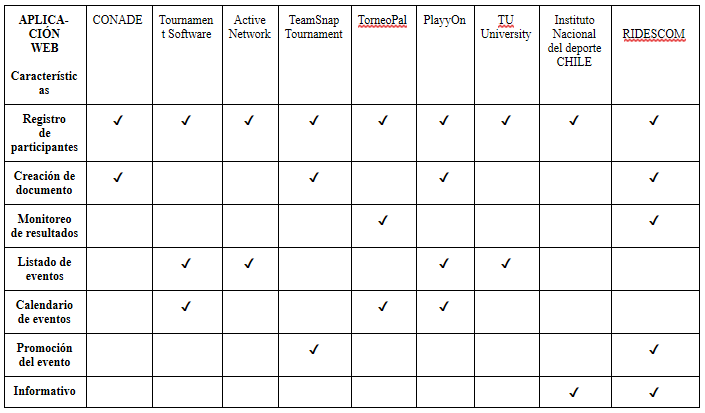
\includegraphics[width=17cm, height=cm]{Imagenes/tablaComparativa}
	\caption{Caracteristicas principales de las páginas similares.}
	\label{tablacomparativa}
\end{figure}

